\documentclass[a4paper]{article}
\usepackage[a4paper, margin=1in]{geometry}
% Some basic packages
\usepackage[utf8]{inputenc}
\usepackage[T1]{fontenc}
\usepackage{textcomp}
\usepackage[dutch]{babel}
\usepackage{url}
\usepackage{graphicx}
\usepackage{float}
\usepackage{booktabs}
\usepackage{enumitem}

\pdfminorversion=7

% Don't indent paragraphs, leave some space between them
\usepackage{parskip}

% Hide page number when page is empty
\usepackage{emptypage}
\usepackage{subcaption}
\usepackage{multicol}
\usepackage{xcolor}

% Other font I sometimes use.
% \usepackage{cmbright}

% Math stuff
\usepackage{amsmath, amsfonts, mathtools, amsthm, amssymb}
% Fancy script capitals
\usepackage{mathrsfs}
\usepackage{cancel}
% Bold math
\usepackage{bm}
% Some shortcuts
\newcommand\N{\ensuremath{\mathbb{N}}}
\newcommand\R{\ensuremath{\mathbb{R}}}
\newcommand\Z{\ensuremath{\mathbb{Z}}}
\renewcommand\O{\ensuremath{\emptyset}}
\newcommand\Q{\ensuremath{\mathbb{Q}}}
\newcommand\C{\ensuremath{\mathbb{C}}}

% Easily typeset systems of equations (French package)
\usepackage{systeme}

% Put x \to \infty below \lim
\let\svlim\lim\def\lim{\svlim\limits}

%Make implies and impliedby shorter
\let\implies\Rightarrow
\let\impliedby\Leftarrow
\let\iff\Leftrightarrow
\let\epsilon\varepsilon

% Add \contra symbol to denote contradiction
\usepackage{stmaryrd} % for \lightning
\newcommand\contra{\scalebox{1.5}{$\lightning$}}

% \let\phi\varphi

% Command for short corrections
% Usage: 1+1=\correct{3}{2}

\definecolor{correct}{HTML}{009900}
\newcommand\correct[2]{\ensuremath{\:}{\color{red}{#1}}\ensuremath{\to }{\color{correct}{#2}}\ensuremath{\:}}
\newcommand\green[1]{{\color{correct}{#1}}}

% horizontal rule
\newcommand\hr{
    \noindent\rule[0.5ex]{\linewidth}{0.5pt}
}

% hide parts
\newcommand\hide[1]{}

% si unitx
\usepackage{siunitx}
\sisetup{locale = FR}

% Environments
\makeatother
% For box around Definition, Theorem, \ldots
\usepackage{mdframed}
\mdfsetup{skipabove=1em,skipbelow=0em}
\theoremstyle{definition}
\newmdtheoremenv[nobreak=true]{definitie}{Definitie}
\newmdtheoremenv[nobreak=true]{eigenschap}{Eigenschap}
\newmdtheoremenv[nobreak=true]{gevolg}{Gevolg}
\newmdtheoremenv[nobreak=true]{lemma}{Lemma}
\newmdtheoremenv[nobreak=true]{propositie}{Propositie}
\newmdtheoremenv[nobreak=true]{stelling}{Stelling}
\newmdtheoremenv[nobreak=true]{wet}{Wet}
\newmdtheoremenv[nobreak=true]{postulaat}{Postulaat}
\newmdtheoremenv{conclusie}{Conclusie}
\newmdtheoremenv{toemaatje}{Toemaatje}
\newmdtheoremenv{vermoeden}{Vermoeden}
\newtheorem*{herhaling}{Herhaling}
\newtheorem*{intermezzo}{Intermezzo}
\newtheorem*{notatie}{Notatie}
\newtheorem*{observatie}{Observatie}
\newtheorem*{oef}{Oefening}
\newtheorem*{opmerking}{Opmerking}
\newtheorem*{praktisch}{Praktisch}
\newtheorem*{probleem}{Probleem}
\newtheorem*{terminologie}{Terminologie}
\newtheorem*{toepassing}{Toepassing}
\newtheorem*{uovt}{UOVT}
\newtheorem*{vb}{Voorbeeld}
\newtheorem*{vraag}{Vraag}

\newmdtheoremenv[nobreak=true]{definition}{Definition}
\newtheorem*{eg}{Example}
\newtheorem*{notation}{Notation}
\newtheorem*{previouslyseen}{As previously seen}
\newtheorem*{remark}{Remark}
\newtheorem*{note}{Note}
\newtheorem*{problem}{Problem}
\newtheorem*{observe}{Observe}
\newtheorem*{property}{Property}
\newtheorem*{intuition}{Intuition}
\newmdtheoremenv[nobreak=true]{prop}{Proposition}
\newmdtheoremenv[nobreak=true]{theorem}{Theorem}
\newmdtheoremenv[nobreak=true]{corollary}{Corollary}

% End example and intermezzo environments with a small diamond (just like proof
% environments end with a small square)
\usepackage{etoolbox}
\AtEndEnvironment{vb}{\null\hfill$\diamond$}%
\AtEndEnvironment{intermezzo}{\null\hfill$\diamond$}%
% \AtEndEnvironment{opmerking}{\null\hfill$\diamond$}%

% Fix some spacing
% http://tex.stackexchange.com/questions/22119/how-can-i-change-the-spacing-before-theorems-with-amsthm
\makeatletter
\def\thm@space@setup{%
  \thm@preskip=\parskip \thm@postskip=0pt
}


% Exercise 
% Usage:
% \oefening{5}
% \suboefening{1}
% \suboefening{2}
% \suboefening{3}
% gives
% Oefening 5
%   Oefening 5.1
%   Oefening 5.2
%   Oefening 5.3
\newcommand{\oefening}[1]{%
    \def\@oefening{#1}%
    \subsection*{Oefening #1}
}

\newcommand{\suboefening}[1]{%
    \subsubsection*{Oefening \@oefening.#1}
}


% \lecture starts a new lecture (les in dutch)
%
% Usage:
% \lecture{1}{di 12 feb 2019 16:00}{Inleiding}
%
% This adds a section heading with the number / title of the lecture and a
% margin paragraph with the date.

% I use \dateparts here to hide the year (2019). This way, I can easily parse
% the date of each lecture unambiguously while still having a human-friendly
% short format printed to the pdf.

\usepackage{xifthen}
\def\testdateparts#1{\dateparts#1\relax}
\def\dateparts#1 #2 #3 #4 #5\relax{
    \marginpar{\small\textsf{\mbox{#1 #2 #3 #5}}}
}

\def\@lecture{}%
\newcommand{\lecture}[3]{
    \ifthenelse{\isempty{#3}}{%
        \def\@lecture{Lecture #1}%
    }{%
        \def\@lecture{Lecture #1: #3}%
    }%
    \subsection*{\@lecture}
    \marginpar{\small\textsf{\mbox{#2}}}
}



% These are the fancy headers
\usepackage{fancyhdr}
\pagestyle{fancy}

% LE: left even
% RO: right odd
% CE, CO: center even, center odd
% My name for when I print my lecture notes to use for an open book exam.
% \fancyhead[LE,RO]{Gilles Castel}

\fancyhead[RO,LE]{\@lecture} % Right odd,  Left even
\fancyhead[RE,LO]{}          % Right even, Left odd

\fancyfoot[RO,LE]{\thepage}  % Right odd,  Left even
\fancyfoot[RE,LO]{}          % Right even, Left odd
\fancyfoot[C]{\leftmark}     % Center

\makeatother




% Todonotes and inline notes in fancy boxes
\usepackage{todonotes}
\usepackage{tcolorbox}

% Make boxes breakable
\tcbuselibrary{breakable}

% Verbetering is correction in Dutch
% Usage: 
% \begin{verbetering}
%     Lorem ipsum dolor sit amet, consetetur sadipscing elitr, sed diam nonumy eirmod
%     tempor invidunt ut labore et dolore magna aliquyam erat, sed diam voluptua. At
%     vero eos et accusam et justo duo dolores et ea rebum. Stet clita kasd gubergren,
%     no sea takimata sanctus est Lorem ipsum dolor sit amet.
% \end{verbetering}
\newenvironment{verbetering}{\begin{tcolorbox}[
    arc=0mm,
    colback=white,
    colframe=green!60!black,
    title=Opmerking,
    fonttitle=\sffamily,
    breakable
]}{\end{tcolorbox}}

% Noot is note in Dutch. Same as 'verbetering' but color of box is different
\newenvironment{noot}[1]{\begin{tcolorbox}[
    arc=0mm,
    colback=white,
    colframe=white!60!black,
    title=#1,
    fonttitle=\sffamily,
    breakable
]}{\end{tcolorbox}}




% Figure support as explained in my blog post.
\usepackage{import}
\usepackage{xifthen}
\usepackage{pdfpages}
\usepackage{transparent}
\newcommand{\incfig}[1]{%
    \def\svgwidth{\columnwidth}
    \import{./figures/}{#1.pdf_tex}
}

% Fix some stuff
% %http://tex.stackexchange.com/questions/76273/multiple-pdfs-with-page-group-included-in-a-single-page-warning
\pdfsuppresswarningpagegroup=1

\title{\Huge{Probability I}\\ Central Limit Theorem}
\author{\huge{Daniel Yu}}
\date{October 8, 2024}

\pdfsuppresswarningpagegroup=1

\begin{document}
\maketitle
\newpage% or \cleardoublepage
% \pdfbookmark[<level>]{<title>}{<dest>}
\tableofcontents
\pagebreak
\section{Review}
Recall\\
Let $X_1$ be any random variable with  $E[X_1] = \mu$ and $Var(X_1) = \sigma^{2}$ and $\{X_i\} $ be an iid sequence. Then,
\[
  Z_n = \frac{1}{n} \sum_{i=1}^{n} X_i, \text{ the average of the first n experiments}
.\] 
\begin{theorem}
  The weak law of large numbers states:
  $Z_n \to \mu$ in probability or equivalently, $\forall \epsilon > 0$:
   \[
     \lim_{n \to \infty} P[\mid Z_n - \mu \mid > \epsilon] = 0
  .\] 
  or equivalently,
  \[
    \lim_{n \to \infty} P[\mid \sum_{i=1}^{n} X_i - n \mu \mid > \epsilon n] = 0
  .\]
  \textbf{what this is saying is that there is emergent determinism, the probability of everything outside of this epsilon, will have eventually have probability 0!}
  \begin{proof}
    First calculate the variance and expected value then apply chebyslev.
    \begin{align*}
      E[Z_n] &= E[\frac{1}{n} \sum_{i=1}^{n} X_i] \\
             &= \frac{1}{n} \sum_{i=1}^{n} E[X_i] \\
             &= \frac{n E[X_i]}{n} \\
             &= \mu
    .\end{align*}
    Then,
    \begin{align*}
      Var(Z_n) &= Var(\frac{1}{n} \sum_{i=1}^{n}X_i) \\
               &= \frac{1}{n}^{2} Var(\sum_{i=1}^{n} X_i) \\
               &\text{ since $X_i$ are iid}\\
               &=  \frac{1}{n}^{2} \sum_{i=1}^{n} Var(X_i) \\
               &= \frac{1}{n}^{2} n \cdot \sigma^{2}\\
               &= \frac{\sigma^{2}}{n}
    .\end{align*}
  Apply chebyslev's inequality.
  \begin{align*}
    P[\mid Z_n - \mu \mid > \epsilon] &\leq \frac{Var(Z_n)}{\epsilon^{2}} \\
                                      &= \frac{\sigma^{2}}{\epsilon^{2}n} \\ 
                                      &\to 0 \text{ as $n \to \infty$}
  .\end{align*}
  \end{proof}
\end{theorem}

\begin{note}{Big Idea}\\
  What is a random variable with variance equal to 0? It is a deterministic random variable. In fact, in the proof above for $\{X_i\}$ we only use iid to show taht the variance goes to 0. More generally, as long as $\{Y_i\}$ to be any sequence of random variables such that 
  \begin{enumerate}
    \item $E[Y_n] \to \mu$ 
    \item $E[Y_n] \to 0$
  \end{enumerate}
  Then we have that $Y_n \to \mu$ in probability. Question, does the other direction hold? I.e. does $Y_n \to \mu$ for some sequence  $\{Y_i\} $ imply that $E[Y_n] \to \mu$ and $Var(Y_n) \to 0$. The answer is no! \\


  Consider $P[A_n = 0] = 1 - \frac{1}{n}, P[A_n = n] = \frac{1}{n}$ so $A_n \to 0$ in probability. The $A_n \to 0$ in probability. However,  $E[A_n] = 0 \cdot (1-\frac{1}{n}) + n \cdot \frac{1}{n} = 1$ and
  \begin{align*}
    Var(A_n) &= E[A_n^{2}] - E[A_n]^{2} \\
             &= \left( n^{2} \cdot \frac{1}{n} + 0^{2} \cdot (1-\frac{1}{n}) \right) - 1^{2} \\
             &= n - 1 \\
             &\to \infty 
  .\end{align*}
\end{note}


\begin{figure}[h]
  \centering
  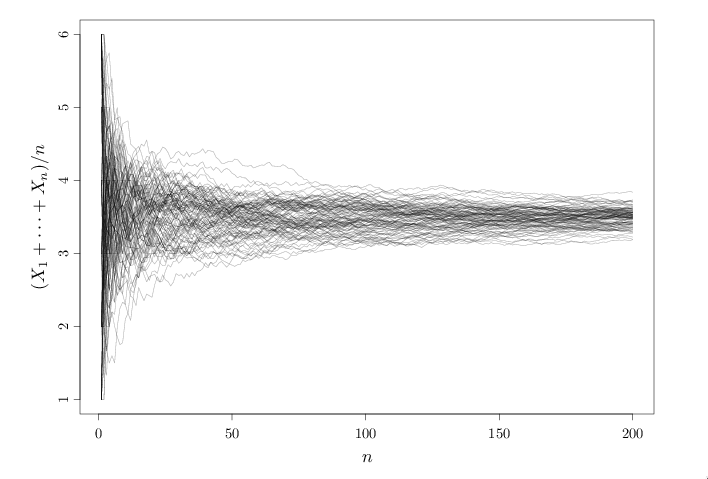
\includegraphics[width=0.8\textwidth]{assets/weak_law_large_numbers_diagram.png}
  \caption{Weak Law of Large Numbers}
  \label{fig:weak_law_large_numbers_diagram}
\end{figure}

\section{Strongest Statement of Weak Law of Large Numbers and its limitations}
\textbf{Can we do better? in case of averages of idd sequences?}

Without loss of generality, let $E[X_1] = 0$ where  $X_i$ are iid. What can we say about?
 \[
   P[\mid \sum_{i=1}^{n} X_i - 0 \cdot \mu \mid]  > \epsilon n^{\frac{2}{3}} 
.\] 
Let's try applying chevslevs inequality again!
\begin{align*}
  P[ \mid \sum_{i=1}^{n} X_i \mid  > \epsilon n^{\frac{2}{3}} ] &\leq \frac{Var(\sum_{i=1}^{n}X_i) }{\epsilon^{2} n^{\frac{2}{3}}} \\
                                                                &=\frac{n \sigma^{2}}{\epsilon^{2} n^{\frac{4}{3}}} \\
                                                                &= \frac{\sigma^{2}}{\epsilon^{2} n^{\frac{1}{3}}} \\
                                                                &\to 0 \text{ as $n \to \infty$}
.\end{align*}
So in general, what $\alpha$ should we choose so that 
\[
  P[\mid \sum_{i=1}^{n} X_i - n \mu \mid > \epsilon n^{\alpha}] \to 0? 
.\] 
Clearly, this works as long as  $\alpha > \frac{1}{2}$ by chevslev's inequality!
\begin{align*}
  P[\mid \sum_{i=1}^{n} X_i - n \mu \mid > \epsilon n^{\alpha}] &\leq \frac{\sigma^{2} n}{\epsilon^{2} n^{2\lapha}}\\
                                                                &= \frac{\sigma^{2}}{\epsilon^{2}} \frac{1}{n^{2 \alpha - 1}}
.\end{align*}
As long as $2 \cdot \alpha -1 > 0$ then the limit is  $0$.
\begin{definition}
  Thus, with $\{X_i\} $ iid. sequence and $E[X_1] = \mu$ and  $Var(X_1) = \sigma^{2}$, then as long as $\alpha > \frac{1}{2}$,
\[
  P[\mid \sum_{i=1}^{n} X_i - n \mu \mid > \epsilon n^{\alpha}] \to 0 
.\] 
\end{definition}

\begin{remark}
  What happens whe $\alpha = \frac{1}{2}$? The weak law of large numbers breaks  down ($ P[\mid \sum_{i=1}^{n} X_i - n \mu \mid > \epsilon n^{\frac{1}{2}}] \leq \frac{\sigma^{2}}{\epsilon^{2}}$. This bound is trivial oftentimes because it is greater than 1 or extremely loose).

As it turns out,
\[
\frac{\mid  \sum_{i=1}^{n} X_i - \mu n\mid }{\sqrt{n}} \not\to c 
.\] in probability, because it is NO LONGER deterministic, it is random!!!

\end{remark}

\begin{remark}
  Our notion of continuity breaks down, we need a new \textbf{topology}
\end{remark}

\section{Convergence in distribution}
\begin{definition}
  Define convergence in distribution as follows. Let $\{Y_n\} $ be a sequence of random variables and $Y$ be a random variable. Then  $Y_n \to Y$ meaning  $Y_n$ converges to  $Y$ in distribution if $\forall E \in \R$,
  \[
    \lim_{n \to \infty} P[Y_n \leq t] = P[Y \leq t] 
  .\] 
  If $Y$ is  discrete, it is sufficient to check
  \[
    \lim_{n \to \infty} P[Y_n = x] = P[Y=x] 
  .\] 
\end{definition}

\begin{note}{Example}\\
  \begin{enumerate}
    \item $P[A_n = 1] = \frac{1}{2} + \frac{1}{n+1}$ 
    \item $P[A_n = -1] = \frac{1}{2} - \frac{1}{n+1}$
  \end{enumerate}
  Then $A_n \to A$ where $A$ is defined as:
   \begin{align*}
     &P[A = 1] =\frac{1}{2} \\
     &P[A=-1] = \frac{1}{2} 
  .\end{align*}
\end{note}
\begin{note}{We would like}\\
  Let $S_n$ to be defined as the set  $\{\frac{-n + 1}{n}, \frac{-n + 2}{n}, \frac{-n+3}{n}, \ldots, \frac{n-1}{n}, \frac{n-1}{n}\}$. Clearly as $n \to \infty$, the  $S_n \to Uniform(-1,1)$ the uniform distribution over  $[-1,1]$. However, how can we should this? \\

   \begin{proof}
     We need to compute $P[S_n \leq t]$. 

\begin{figure}[h]
  \centering
  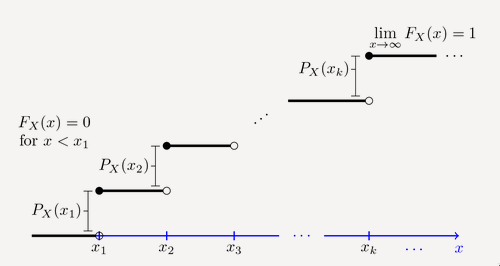
\includegraphics[width=0.8\textwidth]{assets/step_wise_cdf.png}
  \caption{Graph of Probability, where $x_i = \frac{n - i}{n}$, $x_1 = -1$, and  $x_k = 1$}
  \label{fig:step_wise_cdf}
\end{figure} 

  We can see that the number of intervals is $2n-1$.
  \[
    P[S_n \leq 0] = \frac{n+1}{2n-1}
  .\] 
  and,
  \[
    P[S_n \leq t] =\frac{n+1 + \left\lceil nt \right\rceil }{2n-1} \forall t \in [-1,1]
  .\] 
  Thus,
  \[
    \lim_{n \to \infty} P[S_n \leq t] = \frac{1}{2} + \frac{t}{2} = P[Uniform(-1,1) \leq t]
  .\] 
  \end{proof}
\end{note}

\begin{note}{Example}\\
  Take $B_n \sim Bin(n, \frac{2}{n})$. Define $Z$ as:
   \[
  \begin{cases}
    P[Z=0] = \lim_{n \to \infty} P[B_n = 0] \\
    P[Z=1] = \lim_{n \to \infty} P[B_n = 1] \\
 P[Z=2] = \lim_{n \to \infty} P[B_n = 2] \\
 \ldots \\
 P[Z=n] = \lim_{n \to \infty} P[B_n = n] \\
  \end{cases}
  .\] 
  Then, we would like $B_n \to Z$. 

   \begin{proof}
     \begin{align*}
       \lim_{n \to \infty} P[B_n = 0] &= \lim_{n \to \infty} \left( 1 - \frac{2}{n} \right)^{n} \\
                                      &= e^{-2} \\
                                      &= P[Z=0] \\
        P[Z=1] &= \lim_{n \to \infty} \left( \begin{pmatrix} n\\ 1 \end{pmatrix} \frac{n}{2}^{1} \left( 1-\frac{n}{2} \right)^{n-1}  \right) \\
               &= 2 \cdot e^{-2} \\
               &\ldots\\
        P[Z =k] &= \lim_{n \to \infty} \begin{pmatrix} n\\ k \end{pmatrix} \frac{n}{2}^{k} \left( 1-\frac{n}{2} \right)^{n-k} \\
                &= \lim_{n \to \infty} \frac{n \cdot (n-1) \cdot \ldots \cdot (n-k+1)}{k!} \frac{2^{k}}{n^{k}} (1-\frac{2}{n})^{n-k} \\
                &= \frac{2^{k}}{k!} \lim_{n \to \infty} (1-\frac{2}{n})^{k} \cdot \lim_{n \to \infty} \frac{n \cdot (n-1) \cdot \ldots \cdot (n-k+1)}{n^{k}} \\
                &= \frac{e^{-2} \cdot 2^{k}}{k!} \\
                &\sim Poisson(2) 
     .\end{align*}
     So $Z \sim Poiss(2)$. In general, with $B_n \sim Bin(n, \frac{\lambda}{n})$, then $B_n \to Z$ for $Z \sim Possion(\lambda)$
  \end{proof}
\end{note}

\begin{theorem}
  What can we say about the sums of iid random variables? $X_1$ is a random variable with  $E[X_1] = \mu < \infty$,  $Var(X_1) = \sigma^{2} < \infty$, $\{X_i\}$ iid. 
  \[
  \frac{(\sum_{i=1}^{n} X_i - n \mu)}{\sigma \sqrt{n}} \Rightarrow N(0,1)
  .\] 
  Recall that $N(0,1)$ is the random variable with pdf  $\frac{1}{\sqrt{2 \pi}} e^{\frac{-X^{2}}{2}}$. This is the \textbf{central limit theorem}. Equivalently, this means as $n \to \infty$:
  \[
    P[a \leq \frac{(\sum_{i=1}^{n} X_i - n \mu)}{\sigma \sqrt{n}} \leq b] \to P[a \leq N(0,1) \leq b] = \int_{a}^{b} \frac{1}{\sqrt{2 \pi}} e^{\frac{-X^{2}}{2}} dx
  .\] 
\end{theorem}
\begin{lemma}
  A rough approximation is (keyword rough):
  \[
  \sum_{i=1}^{n} X_i \approx n \cdot \mu + \sqrt{n} \cdot \sigma \cdot N(0,1) + \ldots  
  .\] 
  where the other terms grow slower than  $\sqrt{n} $
\end{lemma}
\begin{note}{Important Example}\\
  Consider $W_n$ the random walk (remember that this is a sum of independent walks across timsteps). 
  \begin{enumerate}
    \item What is  $P[W_{10000000000} \geq 0]$? $P[W_{10000000000} \geq 0] \approx \frac{1}{2}$ by symmetry and $E[W_{1000000000}] = 0$ 
    \item What about $P[W_{1000000} \geq 2000]$? $P[W_{1000000} \geq 2000] = P[\frac{\sum_{i=1}^{1000000}W_i - 0 \cdot 1000000}{ 1000} \geq \frac{2000}{1000}] =  P[\frac{\sum_{i=1}^{1000000}W_i}{ 1000} \geq 2]$
    \item Ex: $X$ is a random variable with  $P[X_1 = 2] = \frac{1}{3}, P[X_1 = 4] \frac{1}{2}, P[X_1=8]=\frac{1}{6}$. Approximate $P[\sum_{i=1}^{10000} X_i \leq 39700]$ using central limit theorem. I expect $\sum_{i=1}^{10000} X_i \approx 10,000 E[X]$
      \[
        E[X_1] = 2 \cdot \frac{1}{3} + 4 \cdot \frac{1}{2} + 8 \cdot \frac{1}{6} = 4 
      .\] 
      and, 
      \[
      \sum_{i=1}^{10000} X_i \approx 10,000 \cdot E[X] \approx 40,000
      .\] 
      Now we rescale using the central limit theorem:
      \[
        P[\sum_{i=1}^{10000} X_i \leq 39700] \Rightarrow P[\sum_{i=1}^{10000} X_i - 40000 \leq -300]
      .\]
      Now, compute the variance:
      \[
        Var(X_1) = E[X_1^{2}] - E[X_1]^{2} = 20 - 16 =4
      .\] 
      So,
      \[
        \sigma \cdot \sqrt{n} = \sqrt{Var(X_1)} \cdot \sqrt{n} = 2 \cdot 100 = 200    
      .\] 
      and,
      \[
        P[\sum_{i=1}^{10000} X_i - 40000 \leq -300] \Rightarrow P[\frac{\sum_{i=1}^{10000} X_i - 40000 }{200} \leq -1.5] \approx P[N(0,1) < -1.5] \approx .0668 
      .\] 
      using the calculation.
    \item now consider the sequence of random variables
      \[
      H_n = \frac{\sum_{i=1}^{n} X_i - n \mu}{\sigma \sqrt{n}} = \frac{\sum_{i=1}^{n} (X_i - \mu)}{\sigma \sqrt{n}}
      .\] 
      What is the expected value of $H_n$?
       \[
         E[H_n] = \frac{1}{\sigma \sqrt{n}} [\sum_{i=1}^{n} (E[X_i]) - n \mu] = 0
      .\] 
      What is $E[H_n^{2}]$? 
      \begin{align*}
        E[H_n^{2}] &= \frac{E[(\sum_{i=1}^{n}(X_i - \mu))^{2}]}{\sigma^{2} n} \\
                   &= \frac{1}{\sigma^{2} n} E[\sum_{i=1, j=1}^{n} (X_i - \mu) (X_j - \mu)] \text{ squaring = all possible pairs} \\
                   &= \frac{1}{\sigma^{2}n} \sum_{i=1,j=1}^{n} E[(X_i -\mu)(X_j - \mu)] \\
                   &\text{ this is the Covariance!} \\
                   &= \frac{1}{\sigma^{2}n} \sum_{i=1,j=1}^{n} Cov(X_i, X_j)\\
                   &\text{ when i = j, same RV so cov = var, otherwise covariance of two independent RV is 0!}\\
                   &= \frac{1}{\sigma^{2}n} \left( \sum_{i=j} Var(X_i) + \sum_{i \neq j} 0 \right) \\
                   &= 1
      .\end{align*}
      What about $E[H_n^{3}]$?
      \begin{align*}
        E[H_n^{3}] &= \frac{1}{\sigma^{3}n^{\frac{3}{2}}} \sum_{i,j=1}^{n} E[(X_i -\mu)(X_j - \mu)(X_k -\mu)]\\
                   &\text{ consider case where $i\neq j \neq k$, since $X_i,X_j,X_k$ independent}\\
        E[(X_i -\mu)(X_j - \mu)(X_k -\mu)] &= E[(X_i - \mu)] \cdot E[(X_j - \mu)] \cdot E[(X_k - \mu)] \\
                                           &= 0 \\
                                           &\text{consider case $i=j\neq k$} \\
        E[(X_i - \mu)^{2} (X_k - \mu)] &= E[(X_i - \mu)^{2}] E[(X_k - \mu)] \\
                                       &= 0\\
                                       &\text{ via symmetry this applies to $i \neq j = k$ and  $i = k \neq j$ }\\
                                       &\text{consider case $i = j= k$}\\ 
        E[(X_i - \mu)^{3}] &=  ?
      .\end{align*}
      So,
      \begin{align*}
        E[H_n^{3}] &= \frac{1}{\sigma^{3}n^{\frac{3}{2}}} \sum_{i,j=1}^{n} E[(X_i -\mu)(X_j - \mu)(X_k -\mu)]\\
                   &=  \frac{E[(X_i - \mu)^{3}]}{\sigma^{3} \sqrt{n}}  
                   &\text{ as $n \to \infty$} \\
                   &\to 0
      .\end{align*}
      where $ E[(X_i - \mu)^{3}] $ is known as the third central moment. What about $E[H_n^{4}]$?
      \begin{align*}
        E[H_n^{4}] &= \frac{1}{\sigma^{4}n^{2}} \sum_{i,j,k,l} E[(X_i -\mu)(X_j - \mu)(X_k -\mu) (X_l - \mu)]\\
                   &\text{we know any pairing of $i,j,k,l$ with has at least "one on its own" its own contributes $0$ } \\
                   &= \frac{1}{\sigma^{4}n^{2}} [3 \cdot n (n-1) \cdot E[(X_1 - \mu)^{2} (X_2 - \mu)^{2} + n E[(X_1 - \mu)^{4}] \\
                   &\text{since $x_1,x_2$ independent}\\
        E[(X_1- \mu)^{2}]E[(X_2 - \mu)^{2}] &= E[(X_1 -\mu)^{2}] \cdot E[(X_2 -\mu)^{2}] \\
                                            &= \sigma^{4} \\
        E[H_n^{4}] &= \frac{\sigma^{4} n(n-1)3}{\sigma^{4}n} + \frac{1}{\sigma^{4}n} E[(X_1 - \mu)^{4} ] \\
                   &\text{ as $n \to \infty$} \\
                   &\to 3
      .\end{align*}
      The punchline is:
\begin{table}[h!]
\centering
\begin{tabular}{lcc}
\toprule
Moment & $H_n$ & $N(0,1)$ \\
\midrule
$E[H_n^2]$ & 1 & 1 \\
$E[H_n^3]$ & \to 0 & 0 \\
$E[H_n^4]$ & \to 3 & 3 \\
\bottomrule
\end{tabular}
\caption{Comparison of Moments: $H_n$ vs $N(0,1)$}
\end{table}
  \end{enumerate}
\end{note}


\section{Moment Generating Function}
We need a new tool! 
\begin{definition}
  Given a random variable $X$, the moment generating function of  $X$ is:
   \[
     M_{x}(t) = E[e^{tX}]
  .\] 
  why is this called a moment generating function?
  \begin{enumerate}
    \item $M_X(0) = E[e^{0X}] = 1 = E[X^{0}]$ 
    \item $\frac{d}{dt}M_X(t) = E[\frac{d}{dt}\left( e^{tX} \right)] =E[Xe^{tX}]$
      \[
        \frac{d}{dt} M_X(0) = E[X]
      .\] 
    \item $\frac{d^{2}}{dt^{2}} (M_X(t)) = E[X^{2}e^{tX}]$ 
      \[
        \frac{d^{2}}{dt^{2}} M_X\left( 0 \right) = E[X^{2}]
      .\]
  \end{enumerate}
  Another way of viewing this is that the coefficients of the taylor series expansion of $M_X$ at 0 is precisely the moments of  $X$.
\end{definition}

\begin{lemma}
  $M_{X+Y}(t) = M_X(t) M_Y(t)$ 
  \begin{proof}
    \begin{align*}
      M_{X+Y}(t) &= E[e^{t(X+Y)}] \\
                 &= E[e^{tX} e^{tY}] \\
                 &= E[e^{tX}] E[e^{tY}] \\
                 &= M_X(t) M_Y(t) 
    .\end{align*}
    when $X,Y$ are independent
  \end{proof}
\end{lemma}

\begin{lemma}
  If $c$ constant,
   \[
  M_{cX} (t) = M_X (ct)
  .\] 
  \begin{proof}
    \begin{align*}
      M_{cX}(t) &= E[e^{ctX}] \\
                &= E[e^{(ct)X}] \\
                &= M_X(ct)
    .\end{align*}
  \end{proof}
\end{lemma}

\begin{note}
Let $X = \begin{cases}
  1, P = \frac{1}{2} \\
  0, P = \frac{1}{2} 
\end{cases}$ 
\begin{align*}
  M_X(t) &= E[e^{tX}] \\
         &= e^{1 \cdot t} \cdot \frac{1}{2} + e^{-1 \cdot t} \cdot \frac{1}{2} \\
         &= \frac{e^{t} + e^{-t}}{2} \\
         &= cosh(t)
.\end{align*}
 \[
\frac{d^{n}}{dt^{n}}M_X(t) = \begin{cases}
  \frac{e^{t} - e^{-t}}{2}, \text{ n is odd} \\
  \frac{e^{t} + e^{-t}}{2}, \text{ n is even} 
\end{cases}
.\] 
\[
  E[X^{n}] = \begin{cases}
    0, \text{ if n is even} \\
    1, \text{ if n is odd} 
  \end{cases}
.\] 
\end{note}

\begin{note}
Let $Y \sim \exp(\lambda)$ so the the pdf of  $Y$ is  $\lambda e^{\lambda S}, S \geq 0$.
\begin{align*}
  M_{Y}(t) &= E[e^{tY}] \\
           &= \int_{-\infty}^{\infty} e^{tS} \cdot \lambda e^{-\lambda S} dS \\
           &= \lambda \int_{0}^{\infty} e^{(t - \lambda) S} dS \\
           &= \lambda \cdot \lim_{b \to \infty} \int_{0}^{b} e^{(t - \lambda) S} dS \\
           &= \lambda \cdot \lim_{b \to \infty} [\frac{e^{(t - \lambda) S}}{t-\lambda}]_0^{b}\\
           &= \lambda \lim_{b \to \infty} (\frac{e^{(t-\lambda)b}}{t -\lambda }- \frac{1}{t- \lambda}) 
.\end{align*}
If  \[
\begin{cases}
  t > \lambda , M_{Y}(t) = \frac{\lambda}{\lambda - t} \\
  t \leq \lambda, M_{Y}(t) = \infty
\end{cases}
.\] 
We can see that:
\[
  \frac{d}{dt}^{n} M_{Y}(t) = \frac{n! \cdot \lambda}{(\lambda -t )^{n+1}} \Righarrow E[(\exp(\lambda))^{n}] = \frac{n!}{\lambda^{n}}
.\] 
\end{note}

\begin{theorem}
  $\int_{-\infty}^{\infty} \frac{1}{\sqrt{2 \pi}} e^{\frac{-X^{2}}{2}} dx = I$ i.e. a normal distribution converges.
  \begin{proof}
    \begin{align*}
      I^{2} &= \left( \int_{-\infty}^{\infty} \frac{1}{\sqrt{2} \pi} e^{-\frac{X^{2}}{2}} dx \right) \left(   \int_{-\infty}^{\infty} \frac{1}{\sqrt{2} \pi} e^{-\frac{Y^{2}}{2}} dy \right) \\
            &= \int_{-\infty}^{\infty} \int_{-\infty}^{\infty}  \frac{1}{2 \pi} e^{\frac{-(x^{2} + y^{2})}{2}} dx dy \\
            &\text{ switch to polar} \\
              &= \int_{0}^{2 \pi} \int_{0}^{\infty}  \frac{1}{2 \pi} e^{\frac{-(x^{2} + y^{2})}{2}} r  dr d\theta \\
              &= \int_{0}^{2 \pi} \int_{0}^{\infty}  \frac{1}{2 \pi} e^{\frac{-r^{2}}{2}} r  dr d\theta \\
              &\text{ let $u = e^{\frac{-r^{2}}{2}}$ }\\
              &= \int_{0}^{2 \pi} \int_{0}^{\infty}  \frac{1}{2 \pi} e^{-u} du d\theta\\
              &= \int_{0}^{2\pi} \frac{1}{2\pi} d\theta \\
              &= 1
    .\end{align*}
    Then,
    \[
    \int_{-\infty}^{\infty} \frac{1}{\sqrt{2 \pi}} e^{\frac{-X^{2}}{2}} dx = I  = 1
    .\] 
  \end{proof}
\end{theorem}
\begin{prop}
  $Z \sim N(0,1)$ what is  $M_{Z}(t) = E[e^{tZ}]$?

  \begin{proof}
    
Since $Z$ is normally distributed with mean $0$ and variance $1$, we can express the expectation as an integral:

\[
M_Z(t) = \int_{-\infty}^{\infty} e^{tz} \cdot \frac{1}{\sqrt{2\pi}} e^{-\frac{z^2}{2}} \, dz
\]

This simplifies to:

\[
  M_Z(t) = \frac{1}{\sqrt{2\pi}} \int_{-\infty}^{\infty} e^{\left(tz - \frac{z^2}{2}\right)} \, dz
\]

Now, complete the square in the exponent. The expression inside the exponential is:

\[
tz - \frac{z^2}{2} = -\frac{1}{2}\left(z^2 - 2tz\right) = -\frac{1}{2}\left((z - t)^2 - t^2\right)
\]

Thus, the integral becomes:

\[
  M_Z(t) = \frac{1}{\sqrt{2\pi}} \int_{-\infty}^{\infty} e^{\left(-\frac{(z-t)^2}{2} + \frac{t^2}{2}\right)} \, dz
\]

Factor out the term that does not depend on $z$:

\[
  M_Z(t) = \frac{1}{\sqrt{2\pi}} e^{\left(\frac{t^2}{2}\right)} \int_{-\infty}^{\infty} e^{\left(-\frac{(z-t)^2}{2}\right)} \, dz
\]

Since the remaining integral is just the integral of a Gaussian distribution by the previous thereom we have:

\[
M_Z(t) = \exp\left(\frac{t^2}{2}\right)
\]

Thus, the moment generating function of $Z \sim N(0,1)$ is:

\[
  M_Z(t) = e^{\left(\frac{t^2}{2}\right)}
\]
  \end{proof}
\end{prop}

\begin{theorem}
  \begin{enumerate}
    \item If $M_X(t) = M_{Y}(t)$ then $X,Y$ have the same distribution 
    \item Let  $\{X_n\} $ be a sequence of random variables. If $M_{X_n}(t) \to M_Y(t)$ as $n \to \infty$ then  $X_n \to Y$ in distirubtion. 
  \end{enumerate}
\end{theorem}

\begin{note}{Example}
  Let $z_1 + z_2$ be two independent is $N(0,1)$ what is the distribution of  $\frac{z_1 + z_2}{\sqrt{2} }$.

  \begin{proof}
    \[
Y = \frac{z_1 + z_2}{\sqrt{2}}
\]

The moment generating function (MGF) of $Y$ is:

\[
M_Y(t) = E\left[ e^{tY} \right] = E\left[ e^{t \frac{z_1 + z_2}{\sqrt{2}}} \right] = E\left[ e^{\frac{tz_1}{\sqrt{2}}} \right] \cdot E\left[ e^{\frac{tz_2}{\sqrt{2}}} \right]
\]

Since $z_1$ and $z_2$ are independent $N(0,1)$, their MGF is:

\[
M_{z_i}(t) = \exp\left( \frac{t^2}{2} \right)
\]

Substituting $t \to \frac{t}{\sqrt{2}}$:

\[
M_Y(t) = \exp\left( \frac{t^2}{4} \right) \cdot \exp\left( \frac{t^2}{4} \right) = \exp\left( \frac{t^2}{2} \right)
\]

Thus, $M_Y(t)$ is the MGF of $N(0,1)$, so:

\[
Y \sim N(0,1)
\]
  \end{proof}
\end{note}

\begin{lemma}
  Then $H_n = \frac{\sum_{i=1}^{n} X_i}{\sqrt{n} } \to N(0,1)$ in distribution in the special case $X_i = \pm 1$ with equal probability and  $\{X_i\} $ are iid.
  \begin{proof}
    \begin{align*}
      M_{H_n}(t) &= M_{\frac{\sum_{i=1}^{n} X_i}{\sqrt{n} }} (t) \\
                 &= \Pi_{i=1}^{n} M_{\frac{X_i}{\sqrt{n} }} (t) \\
                 &=  \Pi_{i=1}^{n} M_{X_i} (\frac{t}{\sqrt{n}}) \\
                 &\text{ since $X_i$ are iid} \\
                 &= (M_{X_1}(\frac{t}{\sqrt{n}}))^{n}
    .\end{align*}
    In our case when $X_1=\pm 1$ with probability  $\frac{1}{2}$, then:
    \begin{align*}
      M_{X_1}(t) &= E[e^{tX_1}] \\
                 &= \frac{e^{t}}{2} + \frac{e^{-t}}{2} \\
                 &= \cosh(t)
    .\end{align*}
    Recall that $\cosh(t)$:
    \begin{align*}
      \cosh(t) &= \frac{1}{2} \left( \sum_{n=0}^{\infty} \frac{t^{n}}{n!} \right)  + \frac{1}{2} \sum_{n=0}^{\infty}\frac{(-t)^{n}}{n!} \\
               &= \sum_{n=0}^{\infty} \frac{t^{2n}}{(2n)!} 
    .\end{align*} 
    Then,
    \begin{align*}
      M_{H_n}(t) &= (\cosh(\frac{t}{\sqrt{n} }))^{n} \\
                 &= [1+\frac{\left( \frac{t}{\sqrt{n} } \right)^{2} }{2 } + \frac{\left( \frac{t}{\sqrt{n} } \right)^{4} }{4!} + \ldots]^{n} \\
    .\end{align*}
    Take the limit as $n \to \infty$!
     \[
       \cosh(\frac{t}{\sqrt{n}}) \approx [1 + \frac{t^{2}}{2n} + 0] 
    .\] since the rest of the terms goes to 0 and are much smaller
    Let $L = \lim_{n=\infty} (1+ \frac{t^2}{2n})$.
    \begin{align*}
      \ln(L) &= \ln[\lim_{n\to \infty} (1+\frac{t^2}{2n})^{n}] \\
             &= \lim_{n \to \infty} n \cdot \ln(1+\frac{t^2}{2n})^{n} \\
             &=  
    .\end{align*}
    So $\cosh(\frac{t}{\sqrt{n} })^{n} \to e^{\frac{t^2}{2}} = N(0,1)$ !
  \end{proof}
\end{lemma}
\end{document}
